\section{Task: Donald's Restaurant}\label{sec:donald}

\begin{frame}
	\centering
    \LARGE
    {\nameref{sec:donald}}
\end{frame}

\begin{frame}{A short recap}
    \begin{enumerate}
        \item Orders are submitted as strings in the format: \\
        \enquote{\texttt{<meal\_number>, <servings>}}
        \item Requests for meals are Lists that contain 1 to n Orders
        \item Order strings are split at the comma and used to construct a new Order object
        \item All Orders from one Request are put into an OrderLine object
        \item All Orders in a Request are assigned an increasing index as the order number
        \item Orders are turned into Meals while waiting for a time specified in its recipe
    \end{enumerate}
\end{frame}

\begin{frame}{{\nameref{sec:donald}}}
	\begin{itemize}
		\item Download the zipped project from the workshop repository
        \item Open the project in Netbeans or IntelliJ
        \item Open the class \texttt{Main.java}
	\end{itemize}
    \medskip
    \centering
    \LARGE
    \textbf{\url{https://git.io/vFPQB}}\\
    \normalsize
    \bigskip
    \url{http://reactivex.io/documentation/operators}\\
    RxJava GitHub wiki: \url{https://git.io/vWHZx}\\
    Original Restaurant: \url{https://git.io/vFPby}
\end{frame}

\begin{frame}{{\nameref{sec:donald}}}
    \centering
    \Large
    Create a stream of order strings and print them
\end{frame}

\begin{frame}{{\nameref{sec:donald}}}
    \centering
    \Large
    Parse the order strings into \texttt{Orders} and put them into \texttt{OrderLine}s, then print those
\end{frame}

\begin{frame}{{\nameref{sec:donald}}}
    \centering
    \Large
    Transform every \texttt{Order} in an \texttt{OrderLine} into a \texttt{Meal} and print it
\end{frame}

\begin{frame}{{\nameref{sec:donald}}}
    \centering
    \Large
    Filter out invalid \texttt{Order}s, based on checking their recipe number\\
    Handle exceptions by skipping invalid items
\end{frame}

\begin{frame}{{\nameref{sec:donald}}}
    \centering
    \Large
    Add an incrementing order number to each new \texttt{OrderLine}
\end{frame}

\begin{frame}{{\nameref{sec:donald}}}
	\begin{figure}[h]
		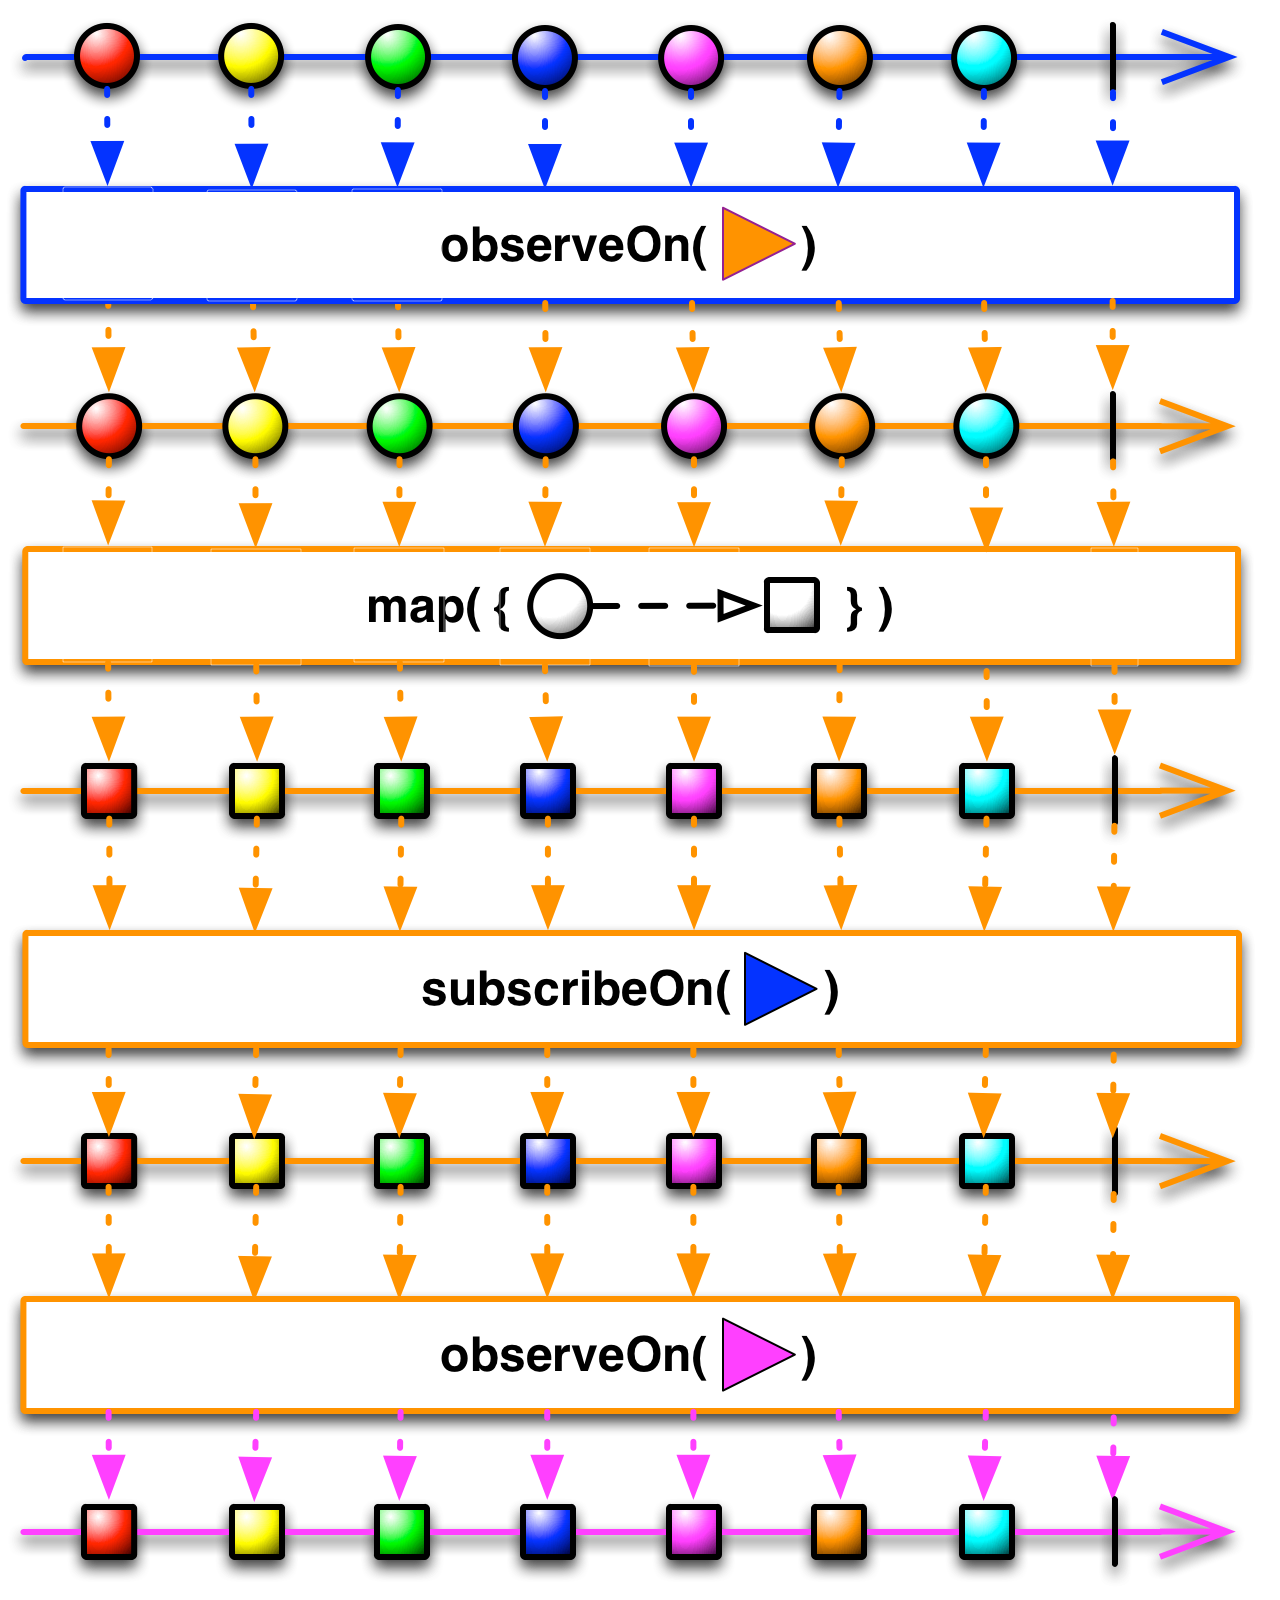
\includegraphics[width=0.6\textwidth,page=1]{gfx/schedulers}
	\end{figure}
\end{frame}

\begin{frame}{{\nameref{sec:donald}}}
	\begin{figure}[h]
		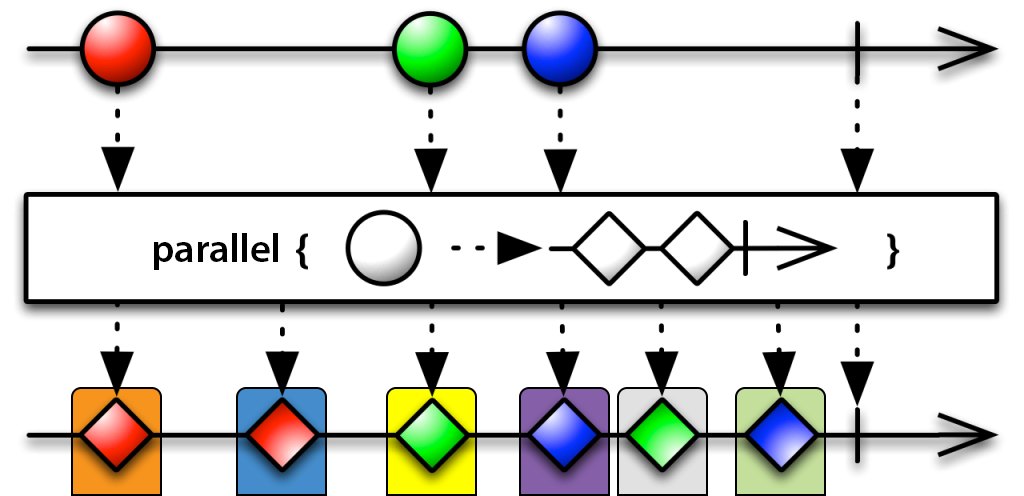
\includegraphics[width=1.0\textwidth,page=1]{gfx/parallel}
	\end{figure}
\end{frame}

\begin{frame}{{\nameref{sec:donald}}}
    \centering
    \Large
    Go multi-threaded by using \texttt{parallel()}
\end{frame}
